\chapter{Results}\label{cha:results}

\section{Depth and ego motion}

\begin{table}[H]
\begin{tabular}{|l|c|c|c|c|c|c|c|c|c|c|}
\hline
 & Net & DS & W & Edge & Norm & Expl & Stat & SSIM & Comb & US \\
\hline
C1 & SL & K & di &  &  & $ \times $ &  &  & avg &  \\
\hline
C2 & SL & K & de &  &  & $ \times $ &  &  & avg &  \\
\hline
C3 & SL & K & de &  &  &  &  &  & avg &  \\
\hline
C4 & SL & K & de &  &  &  & $ \times $ &  & avg &  \\
\hline
C5 & SL & K & de & $ \times $ &  &  & $ \times $ &  & avg &  \\
\hline
C6 & SL & K & de & $ \times $ &  &  & $ \times $ & $ \times $ & min &  \\
\hline
C7 & SL & K & de & $ \times $ & $ \times $ &  & $ \times $ & $ \times $ & min &  \\
\hline
C8 & SL & K & de & $ \times $ & $ \times $ &  & $ \times $ & $ \times $ & min & $ \times $ \\
\hline
C9 & SL & L & de & $ \times $ & $ \times $ &  & $ \times $ & $ \times $ & min & $ \times $ \\
\hline
C10 & M2 & K & de &  &  &  & $ \times $ &  & avg &  \\
\hline
C11 & M2 & K & de & $ \times $ & $ \times $ &  & $ \times $ & $ \times $ & min &  \\
\hline
C12 & M2 & K & de & $ \times $ & $ \times $ &  & $ \times $ & $ \times $ & min & $ \times $ \\
\hline
C13 & M2 & L & de & $ \times $ & $ \times $ &  & $ \times $ & $ \times $ & min & $ \times $ \\
\hline
\end{tabular}
\caption{Different configurations of network architecutes, training datasets and loss terms evaluated to find the best performance}
\label{table:configurations}
\end{table}

\begin{figure}[H]
	\centering
	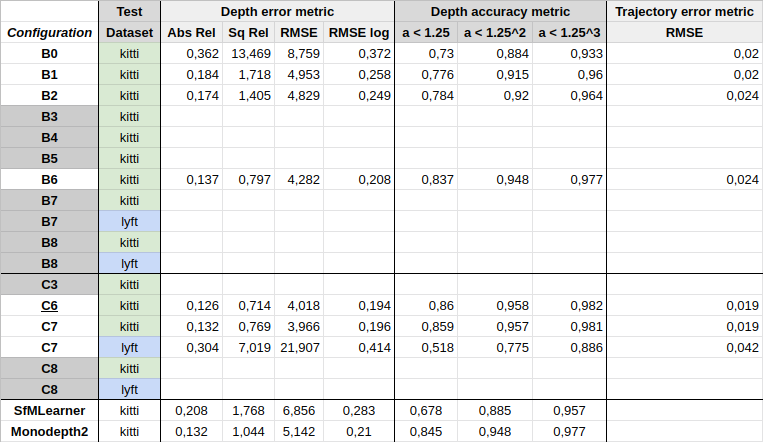
\includegraphics[width=1.0\textwidth]{evaluation}
	\caption{Evaluation metrics when testing the configurations on the testing split of the datasets}
	\label{fig:evaluation}
\end{figure}

\clearpage

\begin{figure}[H]
	\centering
	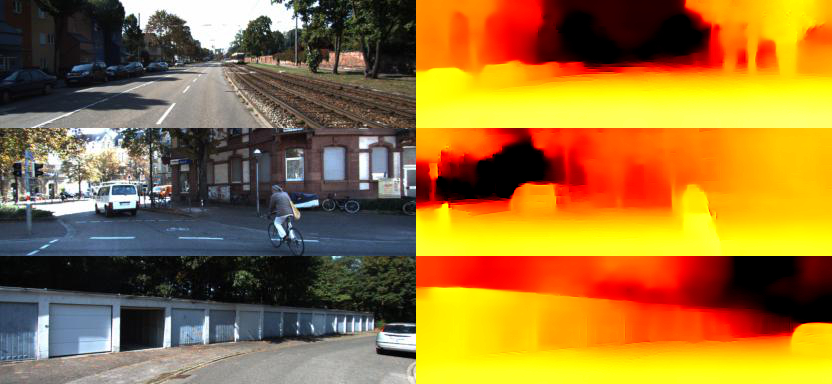
\includegraphics[width=1.0\textwidth]{depthmaps}
	\caption{Examples from the Kitti dataset}
	\label{fig:depthmapskitty}
\end{figure}

%\begin{figure}[H]
%	\centering
%	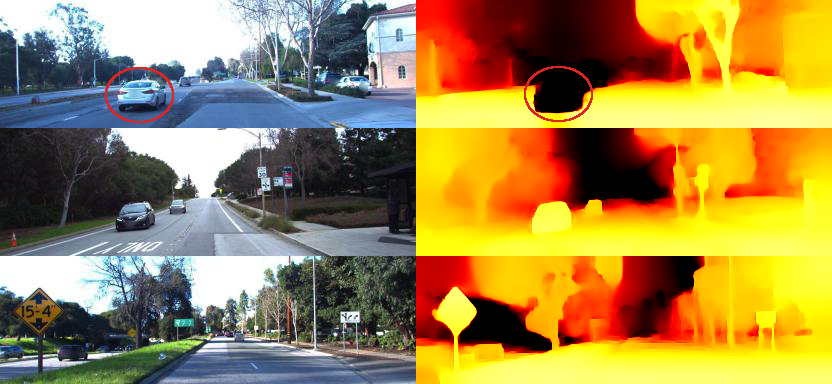
\includegraphics[width=1.0\textwidth]{depthmapslyft}
%	\caption{Examples from the Lyft dataset}
%	\label{fig:depthmaplyft}
%\end{figure}

\begin{figure}[H]
	\centering
	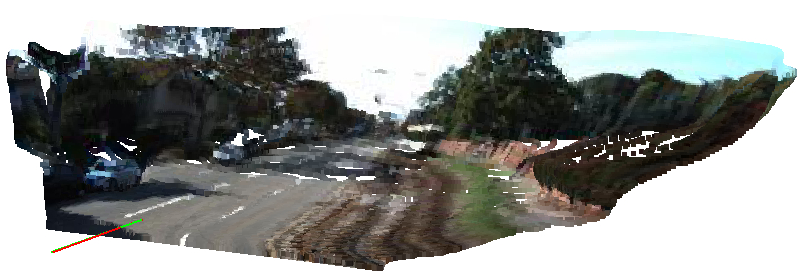
\includegraphics[width=0.8\textwidth]{3drender}
	\caption{3D render of colorized depth map}
	\label{fig:3drender}
\end{figure}

\begin{figure}[H]
	\centering
	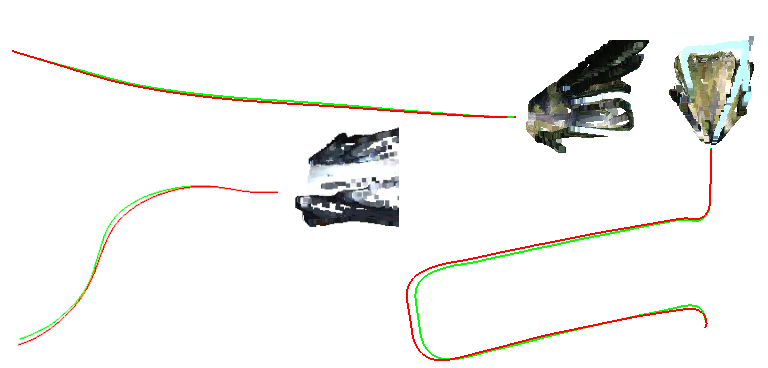
\includegraphics[width=0.8\textwidth]{motion2}
	\caption{3D visualization of the camera movement in three different image sequences. The green lines are the ground truth and the red lines are the predicted camera trajectories.}
	\label{fig:movement}
\end{figure}

\begin{figure}[H]
	\centering
	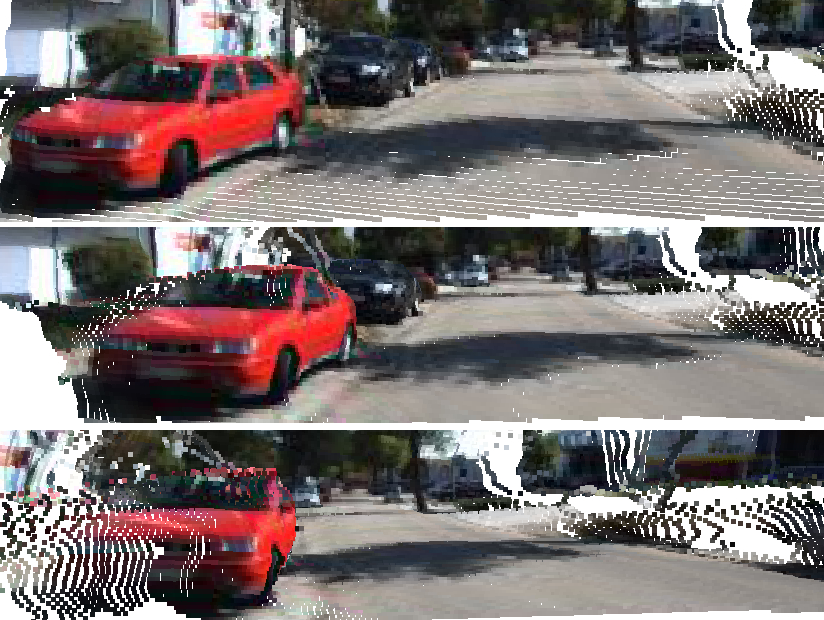
\includegraphics[width=0.8\textwidth]{3dseq}
	\caption{}
	\label{fig:3dseq}
\end{figure}

\section{Keypoint detection}

\begin{figure}[H]
	\centering
	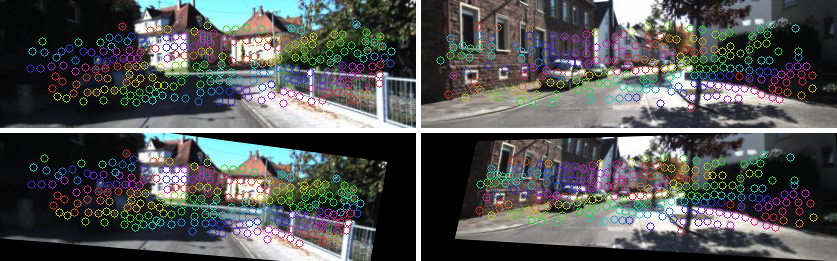
\includegraphics[width=1.0\textwidth]{point1}
	\caption{}
	\label{fig:point1}
\end{figure}

\section{Consensus maximization}